\subsection{Design of a digital IIR filter direct form II}

The delivery of the laboratory required the development of an IIR digital filter with direct form II architecture with the following features:

\begin{itemize}
\item Cut-off frequency $F_{T} = 2 kHz$
\item Number of bits $N_{b} = 10$
\item Filter order $N = 1$
\item Total Harmonic Distorsion $THD \leq -30 dB$
\end{itemize}

\noindent Taking into account the equation that describes the behavior of the IIR filter:

\begin{equation}
y(n) = \sum_{i=0}^N a_{i}x[n-i]  + \sum_{j=1}^N b_{j}y[n-j]
\end{equation}

It is possible to evince the dependence of the filter output as a function of the coefficients $a_{i}$ and $b_{j}$, these are necessary and define the global behavior of the IIR filter, so it was necessary to use tools for their computation. For this purpose Matlab was used, using the scripts made available on the \textit{Portale della didattica}: \textit{my\_filter.m} and \textit{my\_iir\_design.m}.These files made use of the function \textit{butter}, which generates the coefficients of the digital filter with Butterworth response (maximum flat), with the desired filter order and the normalized cut-off frequency compared to the Nyquist frequency. The coefficients quantized at $10 bits$ obtained are as follows:

\begin{itemize}
\item $a = $[512 -82]
\item $b = $[215 215]
\end{itemize}

Matlab's script also generated an implementation of the filter to show the response to two input signals, one in band and the other out of band; it also produced the graph of the frequency response of the filter, as showed in \autoref{fig:IO_signals}:

\begin{figure}[ht]
	\begin{minipage}[b]{0.52\linewidth}
		\centering
		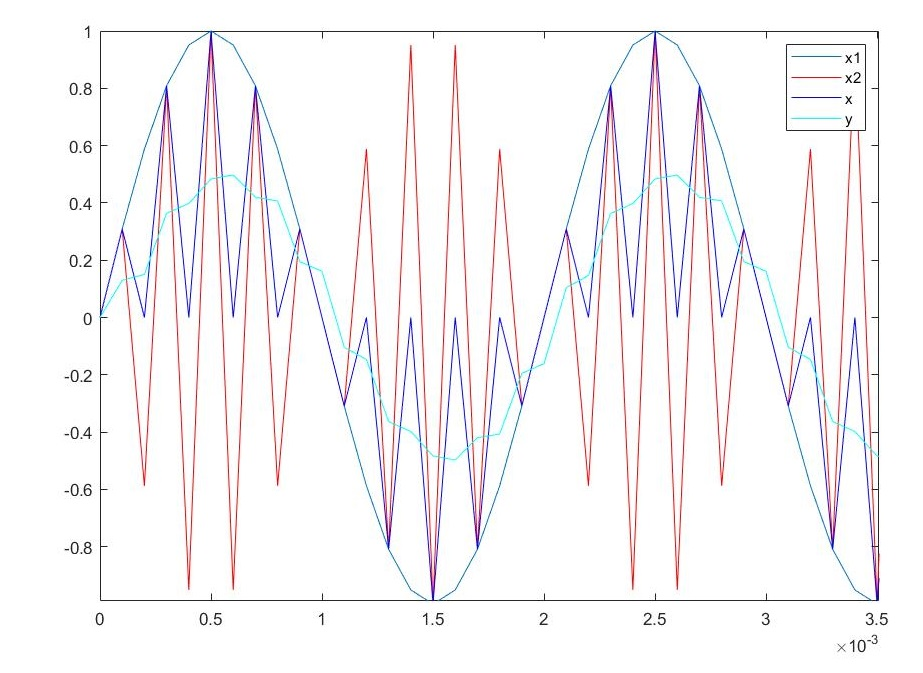
\includegraphics[width=\textwidth]{IIR_IO.jpg}
		\caption{Filter Input and Output Signals}
		\label{fig:IO_signals}
	\end{minipage}
	\hspace{0.1cm}
	\begin{minipage}[b]{0.45\linewidth}
		\centering
		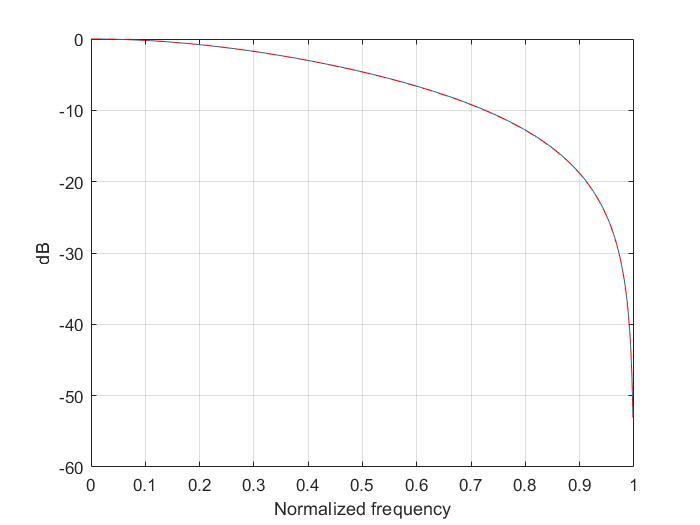
\includegraphics[width=\textwidth]{IIR_responce.jpg}
		\caption{Butterworth response of the IIR filter}.
		\label{fig:Butterworth}
	\end{minipage}
\end{figure}

Signals $x_{1}$ and $x_{2}$ are the in-band signal and the out-of-band signal respectively, the $x$ signal is the average between the two and is given as input to the Matlab program. In fact, as you can see from the output, the filter behaved exactly like a low pass, letting only the low frequency component shift and attenuated to pass.
Then, in \autoref{fig:Butterworth} the Butterworth response is represented as a function of the normalized frequency of the digital IIR filter.